TODO: There should be some blabla. 

\section{Use Case Diagram}

Based on the requirements that were agreed on with the customer, two main use
cases of the system can be found:

\begin{itemize}
\item{Drive out of a perpendicular Parking Lot}
\item{Drive out of a parallel Parking Lot}
\end{itemize}

Both use cases have in common that at the end of the successful process, the
user has to regain the control over its vehicle in a defined way. Additionally,
the user should always have the possibility to interrupt the process and regain
the control over the car, even if the process has not yet finished. Each of the
use cases are triggered by the driver as well as they are supported by various
sensors and control systems.

\begin{figure}
\centering
\captionsetup{justification=centering}
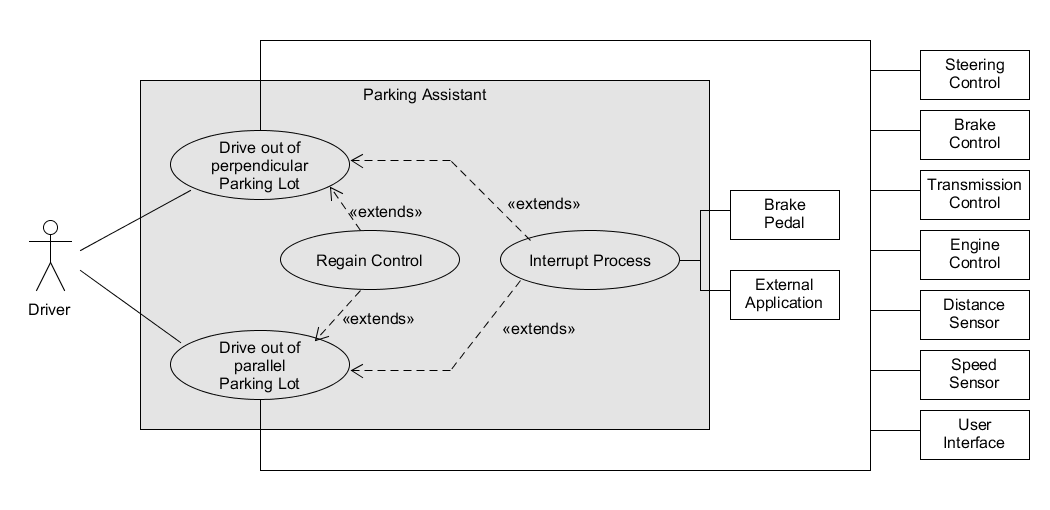
\includegraphics[width=\textwidth]{res/systemAnalysis/UseCase.png}
\caption{Overview of the System's Use Cases}
\label{fig:UseCases}
\end{figure}

\section{Sensor Overview}
To support the presented use cases, the system needs an overview of the cars
surrounding. Six sensors, two of them cameras and 4 of them distance sensors,
are placed in the car to provide this overview. The placement of the sensors can be
retrieved from figure \ref{fig:SensorOverview}.

The sensors that are placed in the middle of the car�s front and rear are
cameras. In many cases cameras are already integrated in the car and provide the
user a realistic image of its surrounding. The distance sensors at the corners
of the bumpers might be radar- or ultrasonic-sensors. Radar sensors have the
advantage, that they might be placed within the bumper and that they are
therefore not visible.

\begin{figure}
\centering
\captionsetup{justification=centering}
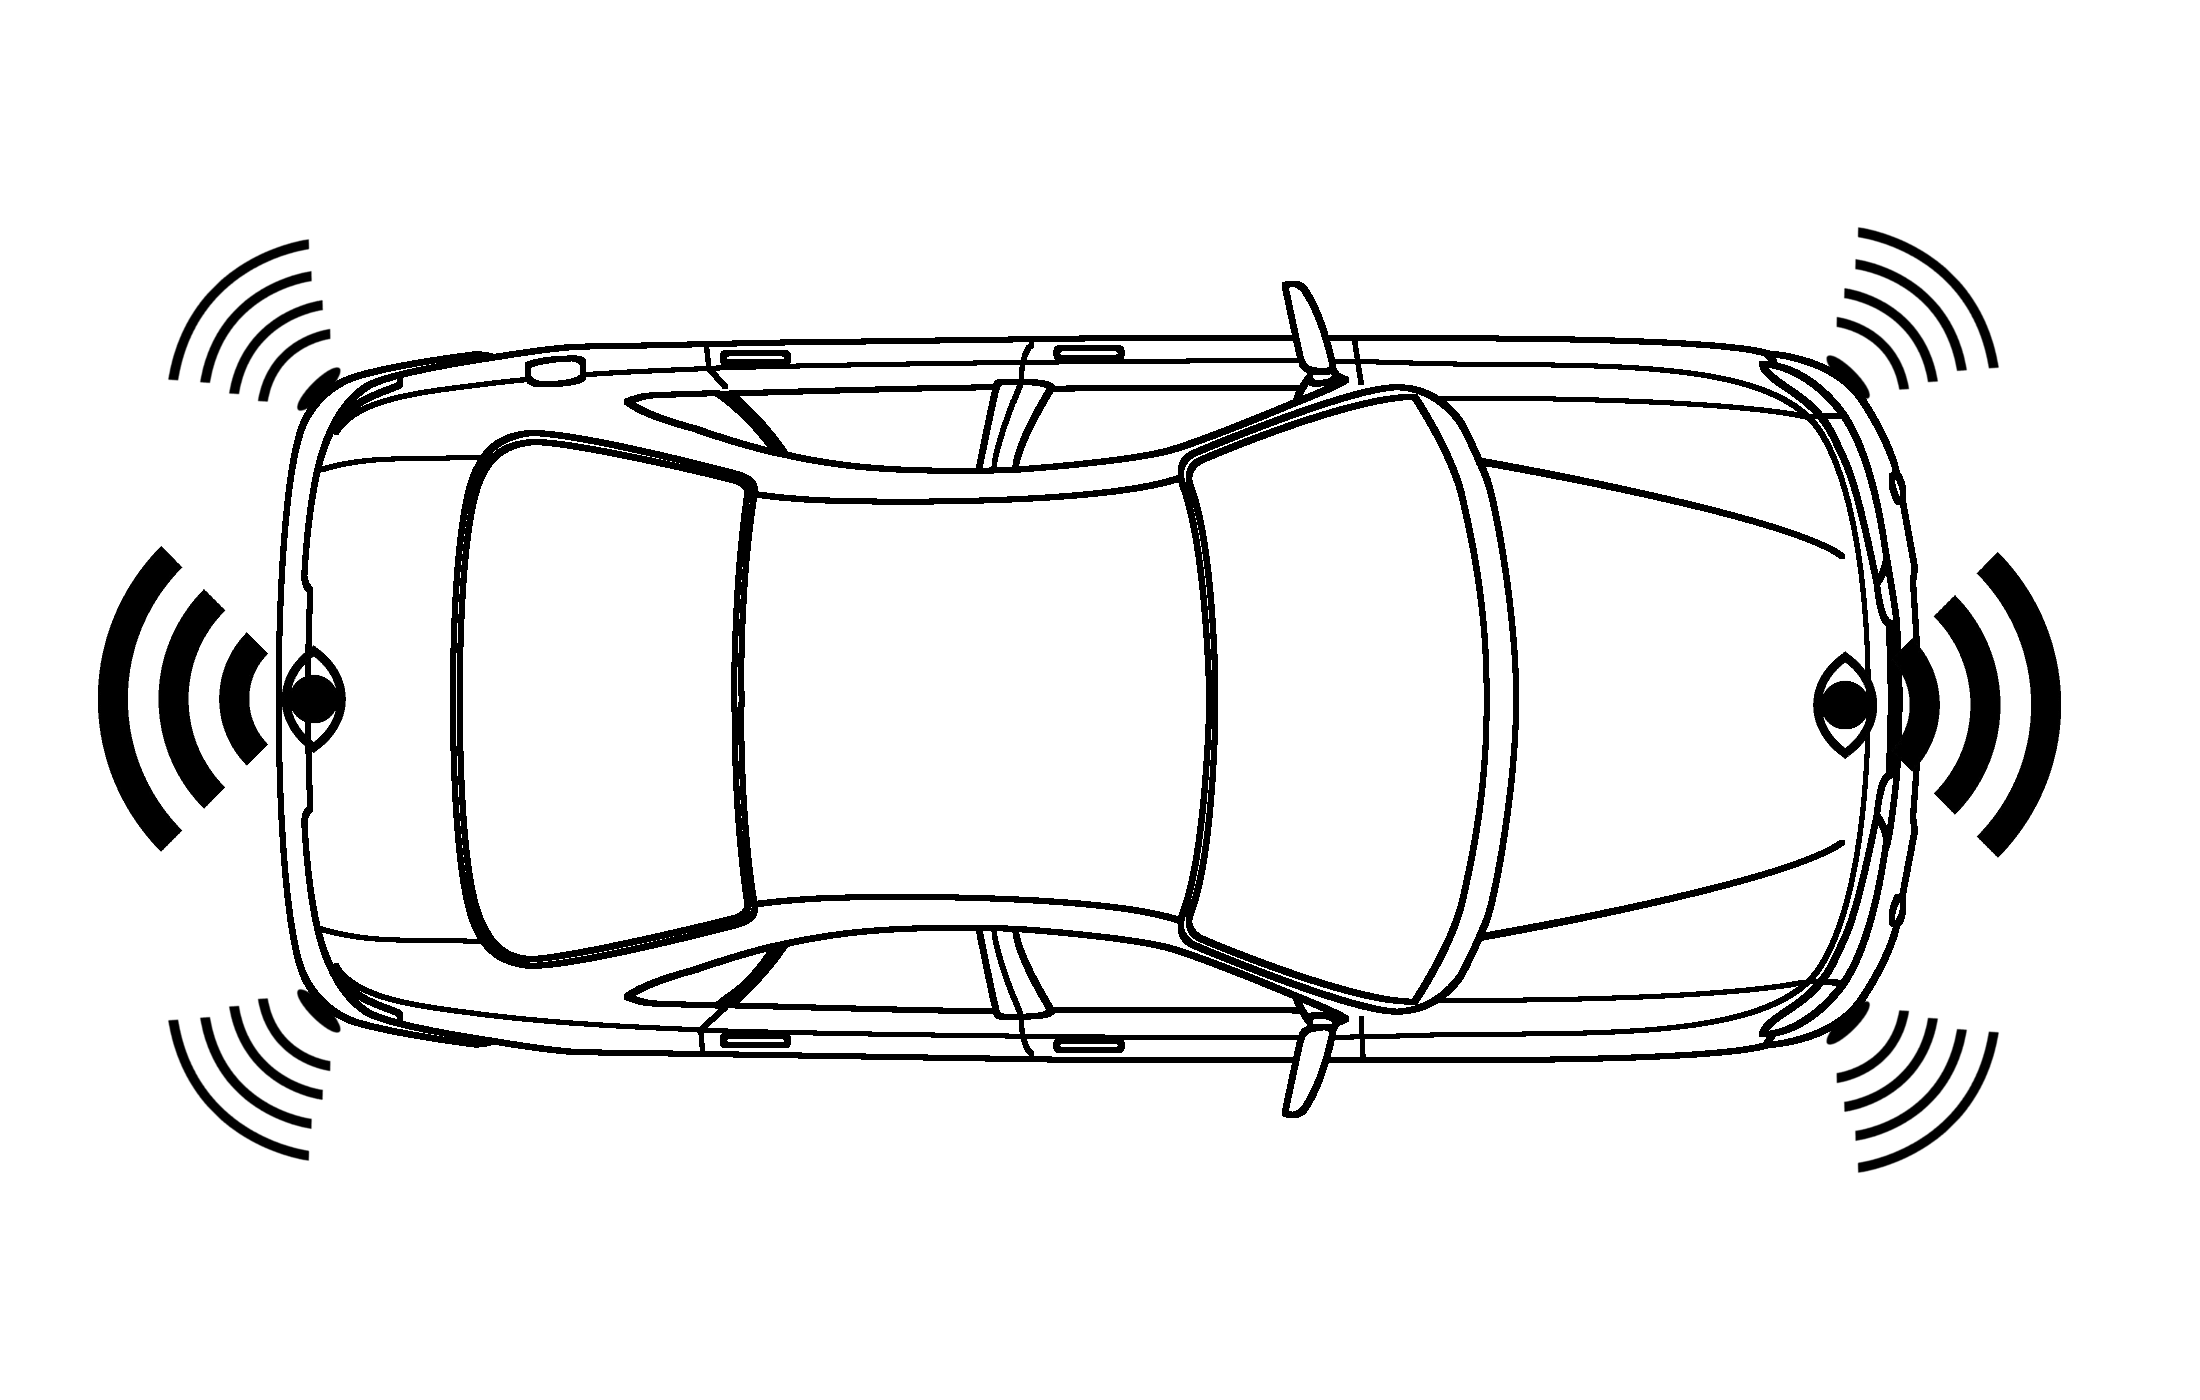
\includegraphics[width=0.75\textwidth]{res/systemAnalysis/SensorOverview.png}
\caption{Overview of the System' Sensors}
\label{fig:SensorOverview}
\end{figure}

\section{Context Diagram}

After the use cases and the required sensors have been found, the context of the
system to develop can be determined (see figure \ref{fig:ContextDiagram}).
Dataflows are depicted with solid arrows while signals that are used to control
the systems are sketched with dashed arrows.

Beside the sensor information, the graphical representation of the process and
the information that is sent to the car�s control systems, there exist two
systems that are used to interrupt the process of leaving a parking lot. If a
driver sits in the car and presses the break pedal, the process will be
interrupted immediately and the driver will regain the control over its vehicle.
If the whole process is controlled remotely without the driver sitting in its
car, the external application that controls the process should act as a dead
man�s switch that is operated by the user. If the signal from this application
is no more retrieved by the system, the process should be interrupted.


\begin{figure}
\centering
\captionsetup{justification=centering}
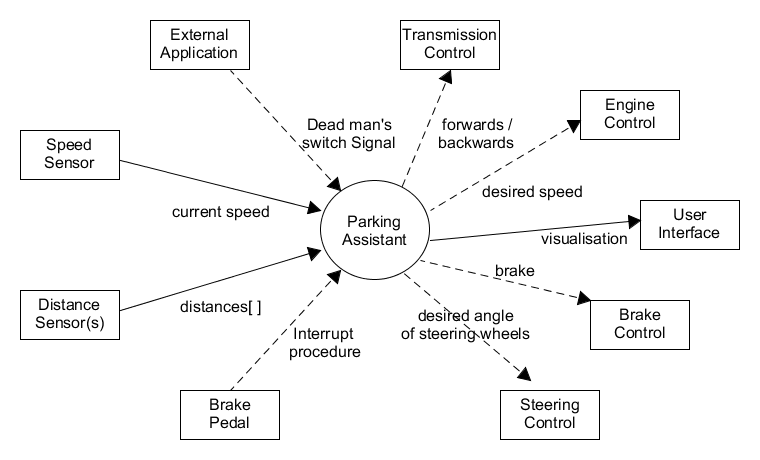
\includegraphics[width=\textwidth]{res/systemAnalysis/ContextDiagram.png}
\caption{Context Diagram of the System}
\label{fig:ContextDiagram}
\end{figure}

\section{Activity Diagram Perpendicular Parking}

\begin{figure}
\centering
\captionsetup{justification=centering}
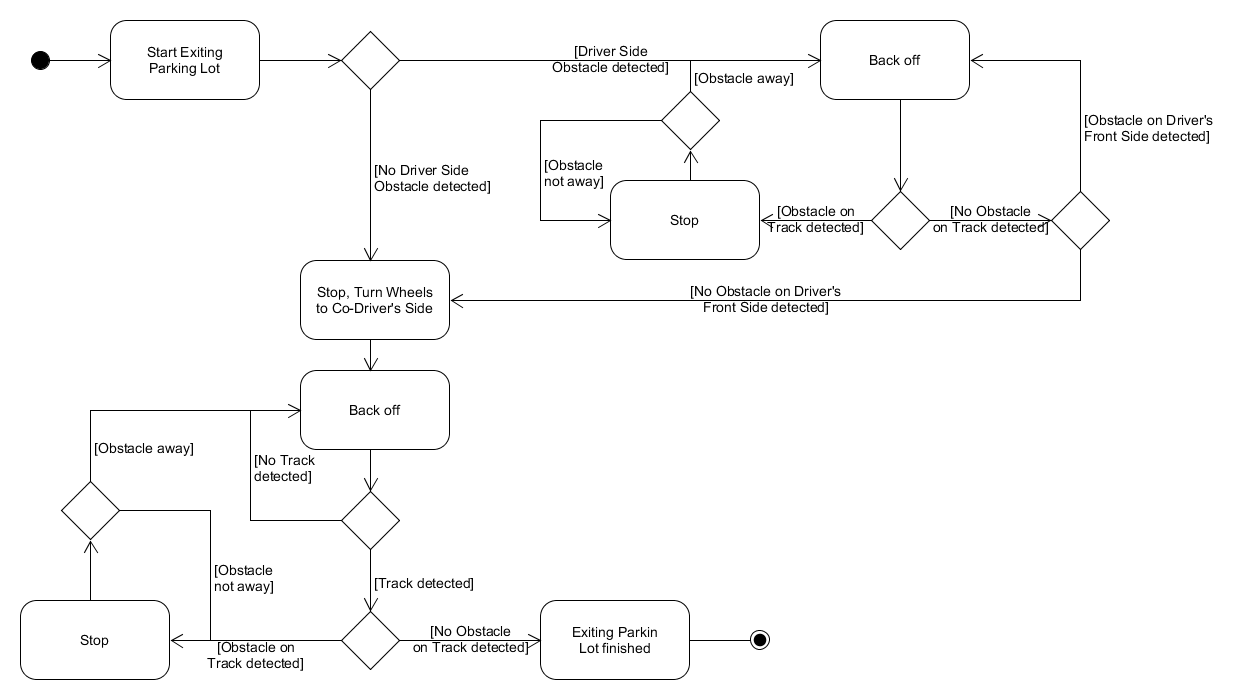
\includegraphics[width=\textwidth]{res/systemAnalysis/ActivityObstacleTransversal.png}
\caption{Algorithm for leaving a perpendicular Parking Situation}
\label{fig:ActivityPerpendicular}
\end{figure}

\section{Activity Diagram Parallel Parking}

\begin{figure}
\centering
\captionsetup{justification=centering}
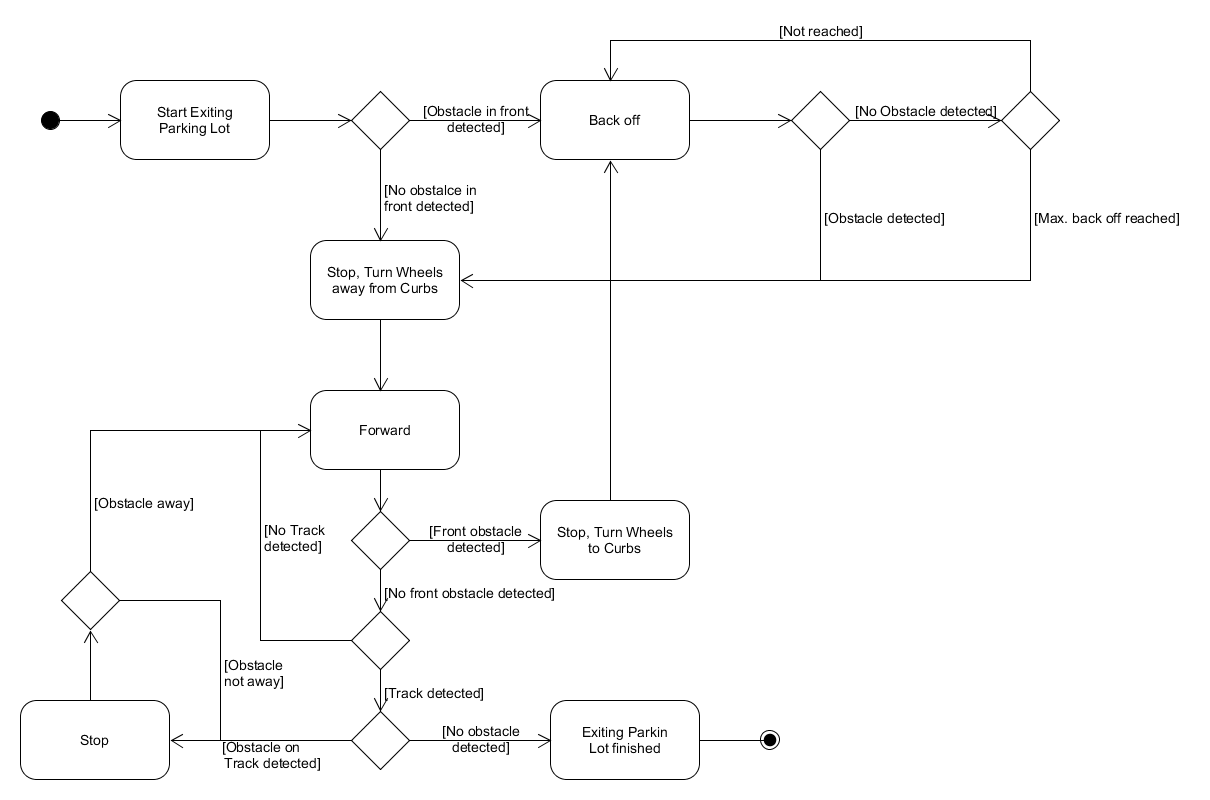
\includegraphics[width=\textwidth]{res/systemAnalysis/ActivityObstacleLenghtwise.png}
\caption{Algorithm for leaving a parallel Parking Situation}
\label{fig:ActivityParallel}
\end{figure}